\documentclass[twoside]{book}

% Packages required by doxygen
\usepackage{fixltx2e}
\usepackage{calc}
\usepackage{doxygen}
\usepackage[export]{adjustbox} % also loads graphicx
\usepackage{graphicx}
\usepackage[utf8]{inputenc}
\usepackage{makeidx}
\usepackage{multicol}
\usepackage{multirow}
\PassOptionsToPackage{warn}{textcomp}
\usepackage{textcomp}
\usepackage[nointegrals]{wasysym}
\usepackage[table]{xcolor}

% Font selection
\usepackage[T1]{fontenc}
\usepackage[scaled=.90]{helvet}
\usepackage{courier}
\usepackage{amssymb}
\usepackage{sectsty}
\renewcommand{\familydefault}{\sfdefault}
\allsectionsfont{%
  \fontseries{bc}\selectfont%
  \color{darkgray}%
}
\renewcommand{\DoxyLabelFont}{%
  \fontseries{bc}\selectfont%
  \color{darkgray}%
}
\newcommand{\+}{\discretionary{\mbox{\scriptsize$\hookleftarrow$}}{}{}}

% Page & text layout
\usepackage{geometry}
\geometry{%
  a4paper,%
  top=2.5cm,%
  bottom=2.5cm,%
  left=2.5cm,%
  right=2.5cm%
}
\tolerance=750
\hfuzz=15pt
\hbadness=750
\setlength{\emergencystretch}{15pt}
\setlength{\parindent}{0cm}
\setlength{\parskip}{3ex plus 2ex minus 2ex}
\makeatletter
\renewcommand{\paragraph}{%
  \@startsection{paragraph}{4}{0ex}{-1.0ex}{1.0ex}{%
    \normalfont\normalsize\bfseries\SS@parafont%
  }%
}
\renewcommand{\subparagraph}{%
  \@startsection{subparagraph}{5}{0ex}{-1.0ex}{1.0ex}{%
    \normalfont\normalsize\bfseries\SS@subparafont%
  }%
}
\makeatother

% Headers & footers
\usepackage{fancyhdr}
\pagestyle{fancyplain}
\fancyhead[LE]{\fancyplain{}{\bfseries\thepage}}
\fancyhead[CE]{\fancyplain{}{}}
\fancyhead[RE]{\fancyplain{}{\bfseries\leftmark}}
\fancyhead[LO]{\fancyplain{}{\bfseries\rightmark}}
\fancyhead[CO]{\fancyplain{}{}}
\fancyhead[RO]{\fancyplain{}{\bfseries\thepage}}
\fancyfoot[LE]{\fancyplain{}{}}
\fancyfoot[CE]{\fancyplain{}{}}
\fancyfoot[RE]{\fancyplain{}{\bfseries\scriptsize Generated by Doxygen }}
\fancyfoot[LO]{\fancyplain{}{\bfseries\scriptsize Generated by Doxygen }}
\fancyfoot[CO]{\fancyplain{}{}}
\fancyfoot[RO]{\fancyplain{}{}}
\renewcommand{\footrulewidth}{0.4pt}
\renewcommand{\chaptermark}[1]{%
  \markboth{#1}{}%
}
\renewcommand{\sectionmark}[1]{%
  \markright{\thesection\ #1}%
}

% Indices & bibliography
\usepackage{natbib}
\usepackage[titles]{tocloft}
\setcounter{tocdepth}{3}
\setcounter{secnumdepth}{5}
\makeindex

% Hyperlinks (required, but should be loaded last)
\usepackage{ifpdf}
\ifpdf
  \usepackage[pdftex,pagebackref=true]{hyperref}
\else
  \usepackage[ps2pdf,pagebackref=true]{hyperref}
\fi
\hypersetup{%
  colorlinks=true,%
  linkcolor=blue,%
  citecolor=blue,%
  unicode%
}

% Custom commands
\newcommand{\clearemptydoublepage}{%
  \newpage{\pagestyle{empty}\cleardoublepage}%
}

\usepackage{caption}
\captionsetup{labelsep=space,justification=centering,font={bf},singlelinecheck=off,skip=4pt,position=top}

%===== C O N T E N T S =====

\begin{document}

% Titlepage & ToC
\hypersetup{pageanchor=false,
             bookmarksnumbered=true,
             pdfencoding=unicode
            }
\pagenumbering{alph}
\begin{titlepage}
\vspace*{7cm}
\begin{center}%
{\Large Doxygen Testing }\\
\vspace*{1cm}
{\large Generated by Doxygen 1.8.13}\\
\end{center}
\end{titlepage}
\clearemptydoublepage
\pagenumbering{roman}
\tableofcontents
\clearemptydoublepage
\pagenumbering{arabic}
\hypersetup{pageanchor=true}

%--- Begin generated contents ---
\chapter{Doxygen}
\label{md_README}
\Hypertarget{md_README}
This repo uses an example class to demonstrate Doxygen and how it helps programmers document our projects using the comments already in our code. This makes documenting our projects faster and more consistent. This is because we only have to document once and don\textquotesingle{}t risk our comments getting lost in translation between viewing the code and documenting it seperately (because the documentation is generates straight from the code).

\section*{\hyperlink{classEmployee}{Employee} Class}

The \hyperlink{classEmployee}{Employee}, \hyperlink{classOfficer}{Officer}, and \hyperlink{classSupervisor}{Supervisor} classes is used to store different employees as objects using code. \hyperlink{classEmployee}{Employee} is the base class, or superclass; \hyperlink{classOfficer}{Officer} and \hyperlink{classSupervisor}{Supervisor} are subclasses of \hyperlink{classEmployee}{Employee}.



\section*{\hyperlink{classOfficer}{Officer} Class}

The \hyperlink{classOfficer}{Officer} class is a subclass of the \hyperlink{classEmployee}{Employee} class. \hyperlink{classOfficer}{Officer} overrides \hyperlink{classEmployee_a01c2c44e15434237db28832f6972e960}{Employee\+::calculate\+Pay()} so the object can properly represent an officer. It has an extra data member, evilness, which is used in the overrided function calculate\+Pay().

\section*{\hyperlink{classSupervisor}{Supervisor} Class}

The \hyperlink{classSupervisor}{Supervisor} class is also a subclass of \hyperlink{classEmployee}{Employee}. It contains an extra data member for tracking the number of people a supervisor object supervises over. That data member is also used in its overrid of \hyperlink{classEmployee_a01c2c44e15434237db28832f6972e960}{Employee\+::calculate\+Pay()}. 
\chapter{Hierarchical Index}
\section{Class Hierarchy}
This inheritance list is sorted roughly, but not completely, alphabetically\+:\begin{DoxyCompactList}
\item \contentsline{section}{Employee}{\pageref{classEmployee}}{}
\begin{DoxyCompactList}
\item \contentsline{section}{Officer}{\pageref{classOfficer}}{}
\item \contentsline{section}{Supervisor}{\pageref{classSupervisor}}{}
\end{DoxyCompactList}
\end{DoxyCompactList}

\chapter{Class Index}
\section{Class List}
Here are the classes, structs, unions and interfaces with brief descriptions\+:\begin{DoxyCompactList}
\item\contentsline{section}{\hyperlink{classEmployee}{Employee} \\*\hyperlink{classEmployee}{Employee} class }{\pageref{classEmployee}}{}
\item\contentsline{section}{\hyperlink{classOfficer}{Officer} }{\pageref{classOfficer}}{}
\item\contentsline{section}{\hyperlink{classSupervisor}{Supervisor} }{\pageref{classSupervisor}}{}
\end{DoxyCompactList}

\chapter{File Index}
\section{File List}
Here is a list of all documented files with brief descriptions\+:\begin{DoxyCompactList}
\item\contentsline{section}{\hyperlink{Employee_8cpp}{Employee.\+cpp} \\*Implementation of \hyperlink{classEmployee}{Employee} }{\pageref{Employee_8cpp}}{}
\item\contentsline{section}{\hyperlink{Employee_8h}{Employee.\+h} \\*\hyperlink{classEmployee}{Employee} class; superclass to supervisor and officer }{\pageref{Employee_8h}}{}
\item\contentsline{section}{\hyperlink{main_8cpp}{main.\+cpp} \\*Main function; facilitates class testing }{\pageref{main_8cpp}}{}
\item\contentsline{section}{\hyperlink{Officer_8cpp}{Officer.\+cpp} \\*\hyperlink{classOfficer}{Officer} implementation }{\pageref{Officer_8cpp}}{}
\item\contentsline{section}{\hyperlink{Officer_8h}{Officer.\+h} \\*\hyperlink{classOfficer}{Officer} class; represents an officer }{\pageref{Officer_8h}}{}
\item\contentsline{section}{\hyperlink{Supervisor_8cpp}{Supervisor.\+cpp} \\*Implementation of \hyperlink{classSupervisor}{Supervisor} class }{\pageref{Supervisor_8cpp}}{}
\item\contentsline{section}{\hyperlink{Supervisor_8h}{Supervisor.\+h} \\*\hyperlink{classSupervisor}{Supervisor} class }{\pageref{Supervisor_8h}}{}
\end{DoxyCompactList}

\chapter{Class Documentation}
\hypertarget{classEmployee}{}\section{Employee Class Reference}
\label{classEmployee}\index{Employee@{Employee}}


\hyperlink{classEmployee}{Employee} class.  




{\ttfamily \#include \char`\"{}Doxygen/\+Employee.\+h\char`\"{}}



Inheritance diagram for Employee\+:
\nopagebreak
\begin{figure}[H]
\begin{center}
\leavevmode
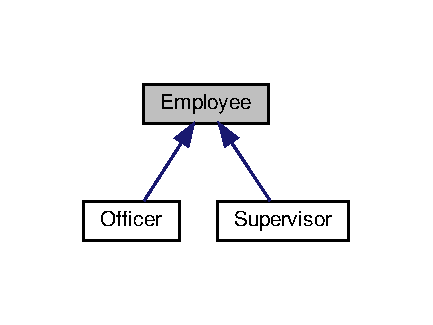
\includegraphics[width=208pt]{classEmployee__inherit__graph}
\end{center}
\end{figure}
\subsection*{Public Member Functions}
\begin{DoxyCompactItemize}
\item 
virtual void \hyperlink{classEmployee_a79556ad700627dba88049f487a34a762}{print} ()
\item 
virtual double \hyperlink{classEmployee_a01c2c44e15434237db28832f6972e960}{calculate\+Pay} ()
\item 
void \hyperlink{classEmployee_a67c345031cf63f515fb09dc675dee5f3}{anniversary} ()
\item 
\hyperlink{classEmployee_a003c7bd08c40924e381eb0750cbb906f}{Employee} ()
\item 
\hyperlink{classEmployee_ad0c935ef9a290a82dcf7865172c90148}{Employee} (int ID, int years, double hourly\+Rate, float hours\+Worked)
\end{DoxyCompactItemize}
\subsection*{Protected Attributes}
\begin{DoxyCompactItemize}
\item 
\mbox{\Hypertarget{classEmployee_ac31134abb9b4004fc015e51ef579b069}\label{classEmployee_ac31134abb9b4004fc015e51ef579b069}} 
double {\bfseries hourly\+Rate}
\item 
\mbox{\Hypertarget{classEmployee_afde35c73d02eb1cfe89e23a80998b42e}\label{classEmployee_afde35c73d02eb1cfe89e23a80998b42e}} 
float {\bfseries hours\+Worked}
\end{DoxyCompactItemize}
\subsection*{Private Attributes}
\begin{DoxyCompactItemize}
\item 
\mbox{\Hypertarget{classEmployee_a832bbae4ee8a704b917f82c4d497bbac}\label{classEmployee_a832bbae4ee8a704b917f82c4d497bbac}} 
int {\bfseries ID}
\item 
\mbox{\Hypertarget{classEmployee_a3e4862d9dfc73becb459a562fa2e25f5}\label{classEmployee_a3e4862d9dfc73becb459a562fa2e25f5}} 
int {\bfseries years}
\end{DoxyCompactItemize}


\subsection{Detailed Description}
\hyperlink{classEmployee}{Employee} class. 

The employee class represents an employee and contains member functions to calculate their pay, view their hourly pay rate, etc. 

\subsection{Constructor \& Destructor Documentation}
\mbox{\Hypertarget{classEmployee_a003c7bd08c40924e381eb0750cbb906f}\label{classEmployee_a003c7bd08c40924e381eb0750cbb906f}} 
\index{Employee@{Employee}!Employee@{Employee}}
\index{Employee@{Employee}!Employee@{Employee}}
\subsubsection{\texorpdfstring{Employee()}{Employee()}\hspace{0.1cm}{\footnotesize\ttfamily [1/2]}}
{\footnotesize\ttfamily Employee\+::\+Employee (\begin{DoxyParamCaption}{ }\end{DoxyParamCaption})}

Default\+Constructor

\begin{DoxyPostcond}{Postcondition}
empty \hyperlink{classEmployee}{Employee} is created 
\end{DoxyPostcond}
\mbox{\Hypertarget{classEmployee_ad0c935ef9a290a82dcf7865172c90148}\label{classEmployee_ad0c935ef9a290a82dcf7865172c90148}} 
\index{Employee@{Employee}!Employee@{Employee}}
\index{Employee@{Employee}!Employee@{Employee}}
\subsubsection{\texorpdfstring{Employee()}{Employee()}\hspace{0.1cm}{\footnotesize\ttfamily [2/2]}}
{\footnotesize\ttfamily Employee\+::\+Employee (\begin{DoxyParamCaption}\item[{int}]{ID,  }\item[{int}]{years,  }\item[{double}]{hourly\+Rate,  }\item[{float}]{hours\+Worked }\end{DoxyParamCaption})}

Parameterized constructor


\begin{DoxyParams}{Parameters}
{\em int} & ID the employee\textquotesingle{}s ID number \\
\hline
{\em int} & years The number of years an employee has worked \\
\hline
{\em double} & hourly\+Rate the wage an employee makes per hour \\
\hline
{\em float} & hours\+Worked the number of hours worked \\
\hline
\end{DoxyParams}
\begin{DoxyPrecond}{Precondition}

\end{DoxyPrecond}
\begin{DoxyPostcond}{Postcondition}
\hyperlink{classEmployee}{Employee} is created with given parameters 
\end{DoxyPostcond}


\subsection{Member Function Documentation}
\mbox{\Hypertarget{classEmployee_a67c345031cf63f515fb09dc675dee5f3}\label{classEmployee_a67c345031cf63f515fb09dc675dee5f3}} 
\index{Employee@{Employee}!anniversary@{anniversary}}
\index{anniversary@{anniversary}!Employee@{Employee}}
\subsubsection{\texorpdfstring{anniversary()}{anniversary()}}
{\footnotesize\ttfamily void Employee\+::anniversary (\begin{DoxyParamCaption}{ }\end{DoxyParamCaption})}

Signifies the employee has been working for another year; increases pay and increments years

\begin{DoxyPrecond}{Precondition}
\hyperlink{classEmployee}{Employee} exists with years and hourly\+Rate 
\end{DoxyPrecond}
\begin{DoxyReturn}{Returns}
void 
\end{DoxyReturn}
\begin{DoxyPostcond}{Postcondition}
hourly\+Rate is increasted 0.\+2\% and years is incremented. 
\end{DoxyPostcond}
\mbox{\Hypertarget{classEmployee_a01c2c44e15434237db28832f6972e960}\label{classEmployee_a01c2c44e15434237db28832f6972e960}} 
\index{Employee@{Employee}!calculate\+Pay@{calculate\+Pay}}
\index{calculate\+Pay@{calculate\+Pay}!Employee@{Employee}}
\subsubsection{\texorpdfstring{calculate\+Pay()}{calculatePay()}}
{\footnotesize\ttfamily double Employee\+::calculate\+Pay (\begin{DoxyParamCaption}{ }\end{DoxyParamCaption})\hspace{0.3cm}{\ttfamily [virtual]}}

Calculates and returns the pay they should revieve based on the hours they worked and hourly wage

\begin{DoxyPrecond}{Precondition}
\hyperlink{classEmployee}{Employee} has a hourly\+Rate and hours\+Worked 
\end{DoxyPrecond}
\begin{DoxyReturn}{Returns}
virtual Can be overriden by subclasses 

double The payment that should be recieved 
\end{DoxyReturn}


Reimplemented in \hyperlink{classOfficer_a1fa1aad39b9e95be7a088990ebf17059}{Officer}, and \hyperlink{classSupervisor_aa37daa89523c08b84ae8141299e036f8}{Supervisor}.



Referenced by Supervisor\+::calculate\+Pay().

\mbox{\Hypertarget{classEmployee_a79556ad700627dba88049f487a34a762}\label{classEmployee_a79556ad700627dba88049f487a34a762}} 
\index{Employee@{Employee}!print@{print}}
\index{print@{print}!Employee@{Employee}}
\subsubsection{\texorpdfstring{print()}{print()}}
{\footnotesize\ttfamily void Employee\+::print (\begin{DoxyParamCaption}{ }\end{DoxyParamCaption})\hspace{0.3cm}{\ttfamily [virtual]}}

Prints out the member variables and more of an employee

\begin{DoxyPrecond}{Precondition}
\hyperlink{classEmployee}{Employee} exists 
\end{DoxyPrecond}
\begin{DoxyReturn}{Returns}
virtual Can be overriden in subclasses 
\end{DoxyReturn}
\begin{DoxyPostcond}{Postcondition}
The employee\textquotesingle{}s information is printed to the console. 
\end{DoxyPostcond}


Reimplemented in \hyperlink{classOfficer_aeadece05a1a0b7fb29bd412830d2e07a}{Officer}, and \hyperlink{classSupervisor_a92483dc9a54904d79b46c6ec4efb3f54}{Supervisor}.



Referenced by Officer\+::print(), and Supervisor\+::print().



The documentation for this class was generated from the following files\+:\begin{DoxyCompactItemize}
\item 
\hyperlink{Employee_8h}{Employee.\+h}\item 
\hyperlink{Employee_8cpp}{Employee.\+cpp}\end{DoxyCompactItemize}

\hypertarget{classOfficer}{}\section{Officer Class Reference}
\label{classOfficer}\index{Officer@{Officer}}


Inheritance diagram for Officer\+:
\nopagebreak
\begin{figure}[H]
\begin{center}
\leavevmode
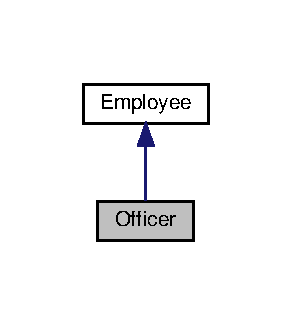
\includegraphics[width=140pt]{classOfficer__inherit__graph}
\end{center}
\end{figure}


Collaboration diagram for Officer\+:
\nopagebreak
\begin{figure}[H]
\begin{center}
\leavevmode
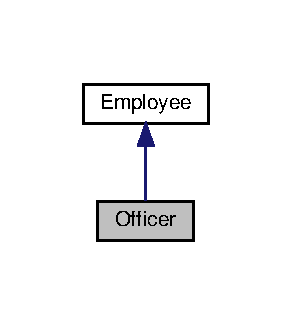
\includegraphics[width=140pt]{classOfficer__coll__graph}
\end{center}
\end{figure}
\subsection*{Public Member Functions}
\begin{DoxyCompactItemize}
\item 
void \hyperlink{classOfficer_aeadece05a1a0b7fb29bd412830d2e07a}{print} ()
\item 
double \hyperlink{classOfficer_a1fa1aad39b9e95be7a088990ebf17059}{calculate\+Pay} ()
\item 
\hyperlink{classOfficer_a80ac1e36a3f36c3a7e12b5dc9320ad89}{Officer} ()
\item 
\hyperlink{classOfficer_ac75c45d6e8628606278cb4ce6596f67f}{Officer} (int ID, int years, double hourly\+Rate, float hours\+Worked, double evilness)
\end{DoxyCompactItemize}
\subsection*{Private Attributes}
\begin{DoxyCompactItemize}
\item 
\mbox{\Hypertarget{classOfficer_a63465c5f16e8148e5bc0a3bb4ecd1781}\label{classOfficer_a63465c5f16e8148e5bc0a3bb4ecd1781}} 
double {\bfseries evilness}
\end{DoxyCompactItemize}
\subsection*{Additional Inherited Members}


\subsection{Constructor \& Destructor Documentation}
\mbox{\Hypertarget{classOfficer_a80ac1e36a3f36c3a7e12b5dc9320ad89}\label{classOfficer_a80ac1e36a3f36c3a7e12b5dc9320ad89}} 
\index{Officer@{Officer}!Officer@{Officer}}
\index{Officer@{Officer}!Officer@{Officer}}
\subsubsection{\texorpdfstring{Officer()}{Officer()}\hspace{0.1cm}{\footnotesize\ttfamily [1/2]}}
{\footnotesize\ttfamily Officer\+::\+Officer (\begin{DoxyParamCaption}{ }\end{DoxyParamCaption})}

Default Constructor

\begin{DoxyPrecond}{Precondition}

\end{DoxyPrecond}
\begin{DoxyPostcond}{Postcondition}
empty officer object is created 
\end{DoxyPostcond}
\mbox{\Hypertarget{classOfficer_ac75c45d6e8628606278cb4ce6596f67f}\label{classOfficer_ac75c45d6e8628606278cb4ce6596f67f}} 
\index{Officer@{Officer}!Officer@{Officer}}
\index{Officer@{Officer}!Officer@{Officer}}
\subsubsection{\texorpdfstring{Officer()}{Officer()}\hspace{0.1cm}{\footnotesize\ttfamily [2/2]}}
{\footnotesize\ttfamily Officer\+::\+Officer (\begin{DoxyParamCaption}\item[{int}]{ID,  }\item[{int}]{years,  }\item[{double}]{hourly\+Rate,  }\item[{float}]{hours\+Worked,  }\item[{double}]{evilness }\end{DoxyParamCaption})}

Parameterized Constructor


\begin{DoxyParams}{Parameters}
{\em int} & ID ID number of officer \\
\hline
{\em int} & years number of years the officer has worked \\
\hline
{\em double} & hourly\+Rate The officer\textquotesingle{}s hourly pay rate \\
\hline
{\em float} & hours\+Worked the number of hours worked \\
\hline
{\em double} & evilness the evilness of the officer; proportional to pay \\
\hline
\end{DoxyParams}
\begin{DoxyPrecond}{Precondition}

\end{DoxyPrecond}
\begin{DoxyPostcond}{Postcondition}
\hyperlink{classOfficer}{Officer} with given parameters created 
\end{DoxyPostcond}


\subsection{Member Function Documentation}
\mbox{\Hypertarget{classOfficer_a1fa1aad39b9e95be7a088990ebf17059}\label{classOfficer_a1fa1aad39b9e95be7a088990ebf17059}} 
\index{Officer@{Officer}!calculate\+Pay@{calculate\+Pay}}
\index{calculate\+Pay@{calculate\+Pay}!Officer@{Officer}}
\subsubsection{\texorpdfstring{calculate\+Pay()}{calculatePay()}}
{\footnotesize\ttfamily double Officer\+::calculate\+Pay (\begin{DoxyParamCaption}{ }\end{DoxyParamCaption})\hspace{0.3cm}{\ttfamily [virtual]}}

Calculates the pay of an officer.

\begin{DoxyPrecond}{Precondition}
\hyperlink{classOfficer}{Officer} exists with hourly\+Rate, evilness and hourse\+Worked 
\end{DoxyPrecond}
\begin{DoxyReturn}{Returns}
double Returns the pay they should receive 
\end{DoxyReturn}
\begin{DoxyPostcond}{Postcondition}
The payment is returned 
\end{DoxyPostcond}


Reimplemented from \hyperlink{classEmployee_a01c2c44e15434237db28832f6972e960}{Employee}.

\mbox{\Hypertarget{classOfficer_aeadece05a1a0b7fb29bd412830d2e07a}\label{classOfficer_aeadece05a1a0b7fb29bd412830d2e07a}} 
\index{Officer@{Officer}!print@{print}}
\index{print@{print}!Officer@{Officer}}
\subsubsection{\texorpdfstring{print()}{print()}}
{\footnotesize\ttfamily void Officer\+::print (\begin{DoxyParamCaption}{ }\end{DoxyParamCaption})\hspace{0.3cm}{\ttfamily [virtual]}}

Print out the officer\textquotesingle{}s data

\begin{DoxyPrecond}{Precondition}
An officer object exists 
\end{DoxyPrecond}
\begin{DoxyReturn}{Returns}
void 
\end{DoxyReturn}
\begin{DoxyPostcond}{Postcondition}
The officer\textquotesingle{}s data is written to the console 
\end{DoxyPostcond}


Reimplemented from \hyperlink{classEmployee_a79556ad700627dba88049f487a34a762}{Employee}.



The documentation for this class was generated from the following files\+:\begin{DoxyCompactItemize}
\item 
\hyperlink{Officer_8h}{Officer.\+h}\item 
\hyperlink{Officer_8cpp}{Officer.\+cpp}\end{DoxyCompactItemize}

\hypertarget{classSupervisor}{}\section{Supervisor Class Reference}
\label{classSupervisor}\index{Supervisor@{Supervisor}}


Inheritance diagram for Supervisor\+:
\nopagebreak
\begin{figure}[H]
\begin{center}
\leavevmode
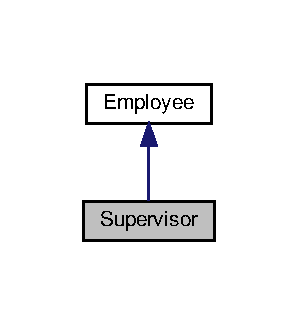
\includegraphics[width=143pt]{classSupervisor__inherit__graph}
\end{center}
\end{figure}


Collaboration diagram for Supervisor\+:
\nopagebreak
\begin{figure}[H]
\begin{center}
\leavevmode
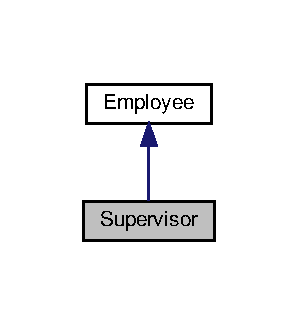
\includegraphics[width=143pt]{classSupervisor__coll__graph}
\end{center}
\end{figure}
\subsection*{Public Member Functions}
\begin{DoxyCompactItemize}
\item 
void \hyperlink{classSupervisor_a92483dc9a54904d79b46c6ec4efb3f54}{print} ()
\item 
double \hyperlink{classSupervisor_aa37daa89523c08b84ae8141299e036f8}{calculate\+Pay} ()
\item 
\hyperlink{classSupervisor_a9d7eafc36b5429092ba0f758bc7841c4}{Supervisor} ()
\item 
\hyperlink{classSupervisor_a02d9245744652deb20e9408001d6ed3b}{Supervisor} (int ID, int years, double hourly\+Rate, float hours\+Worked, int num\+Supervised)
\end{DoxyCompactItemize}
\subsection*{Private Attributes}
\begin{DoxyCompactItemize}
\item 
\mbox{\Hypertarget{classSupervisor_af8b7097d8147c93a68d1f63c5b898797}\label{classSupervisor_af8b7097d8147c93a68d1f63c5b898797}} 
int {\bfseries num\+Supervised}
\end{DoxyCompactItemize}
\subsection*{Additional Inherited Members}


\subsection{Constructor \& Destructor Documentation}
\mbox{\Hypertarget{classSupervisor_a9d7eafc36b5429092ba0f758bc7841c4}\label{classSupervisor_a9d7eafc36b5429092ba0f758bc7841c4}} 
\index{Supervisor@{Supervisor}!Supervisor@{Supervisor}}
\index{Supervisor@{Supervisor}!Supervisor@{Supervisor}}
\subsubsection{\texorpdfstring{Supervisor()}{Supervisor()}\hspace{0.1cm}{\footnotesize\ttfamily [1/2]}}
{\footnotesize\ttfamily Supervisor\+::\+Supervisor (\begin{DoxyParamCaption}{ }\end{DoxyParamCaption})}

Default constructor

\begin{DoxyPrecond}{Precondition}

\end{DoxyPrecond}
\begin{DoxyPostcond}{Postcondition}
\hyperlink{classSupervisor}{Supervisor} created 
\end{DoxyPostcond}
\mbox{\Hypertarget{classSupervisor_a02d9245744652deb20e9408001d6ed3b}\label{classSupervisor_a02d9245744652deb20e9408001d6ed3b}} 
\index{Supervisor@{Supervisor}!Supervisor@{Supervisor}}
\index{Supervisor@{Supervisor}!Supervisor@{Supervisor}}
\subsubsection{\texorpdfstring{Supervisor()}{Supervisor()}\hspace{0.1cm}{\footnotesize\ttfamily [2/2]}}
{\footnotesize\ttfamily Supervisor\+::\+Supervisor (\begin{DoxyParamCaption}\item[{int}]{ID,  }\item[{int}]{years,  }\item[{double}]{hourly\+Rate,  }\item[{float}]{hours\+Worked,  }\item[{int}]{num\+Supervised }\end{DoxyParamCaption})}

Parameterised Constructor


\begin{DoxyParams}{Parameters}
{\em int} & ID ID number of supervisor \\
\hline
{\em int} & years number of years supervisor has worked \\
\hline
{\em double} & hourly\+Rate the hourly pay rate of supervisor \\
\hline
{\em float} & hours\+Worked num of hours worked \\
\hline
{\em int} & num\+Supervised number of people supervised by a supervisor \\
\hline
\end{DoxyParams}
\begin{DoxyPrecond}{Precondition}

\end{DoxyPrecond}
\begin{DoxyPostcond}{Postcondition}
\hyperlink{classSupervisor}{Supervisor} object created with given data 
\end{DoxyPostcond}


\subsection{Member Function Documentation}
\mbox{\Hypertarget{classSupervisor_aa37daa89523c08b84ae8141299e036f8}\label{classSupervisor_aa37daa89523c08b84ae8141299e036f8}} 
\index{Supervisor@{Supervisor}!calculate\+Pay@{calculate\+Pay}}
\index{calculate\+Pay@{calculate\+Pay}!Supervisor@{Supervisor}}
\subsubsection{\texorpdfstring{calculate\+Pay()}{calculatePay()}}
{\footnotesize\ttfamily double Supervisor\+::calculate\+Pay (\begin{DoxyParamCaption}{ }\end{DoxyParamCaption})\hspace{0.3cm}{\ttfamily [virtual]}}

Calculates the pay a supervisor should receive

\begin{DoxyPrecond}{Precondition}
\hyperlink{classSupervisor}{Supervisor} exists with data 
\end{DoxyPrecond}
\begin{DoxyReturn}{Returns}
double Returns the amount the supervisor should be paid; considers num of people supervised 
\end{DoxyReturn}
\begin{DoxyPostcond}{Postcondition}

\end{DoxyPostcond}


Reimplemented from \hyperlink{classEmployee_a01c2c44e15434237db28832f6972e960}{Employee}.

\mbox{\Hypertarget{classSupervisor_a92483dc9a54904d79b46c6ec4efb3f54}\label{classSupervisor_a92483dc9a54904d79b46c6ec4efb3f54}} 
\index{Supervisor@{Supervisor}!print@{print}}
\index{print@{print}!Supervisor@{Supervisor}}
\subsubsection{\texorpdfstring{print()}{print()}}
{\footnotesize\ttfamily void Supervisor\+::print (\begin{DoxyParamCaption}{ }\end{DoxyParamCaption})\hspace{0.3cm}{\ttfamily [virtual]}}

Prints out a \hyperlink{classSupervisor}{Supervisor}\textquotesingle{}s data

\begin{DoxyPrecond}{Precondition}
\hyperlink{classSupervisor}{Supervisor} exists with data 
\end{DoxyPrecond}
\begin{DoxyReturn}{Returns}
void 
\end{DoxyReturn}
\begin{DoxyPostcond}{Postcondition}
\hyperlink{classSupervisor}{Supervisor} data written to console 
\end{DoxyPostcond}


Reimplemented from \hyperlink{classEmployee_a79556ad700627dba88049f487a34a762}{Employee}.



The documentation for this class was generated from the following files\+:\begin{DoxyCompactItemize}
\item 
\hyperlink{Supervisor_8h}{Supervisor.\+h}\item 
\hyperlink{Supervisor_8cpp}{Supervisor.\+cpp}\end{DoxyCompactItemize}

\chapter{File Documentation}
\hypertarget{Employee_8cpp}{}\section{Employee.\+cpp File Reference}
\label{Employee_8cpp}\index{Employee.\+cpp@{Employee.\+cpp}}


Implementation of \hyperlink{classEmployee}{Employee}.  


{\ttfamily \#include \char`\"{}Employee.\+h\char`\"{}}\newline
{\ttfamily \#include $<$iostream$>$}\newline
Include dependency graph for Employee.\+cpp\+:
\nopagebreak
\begin{figure}[H]
\begin{center}
\leavevmode
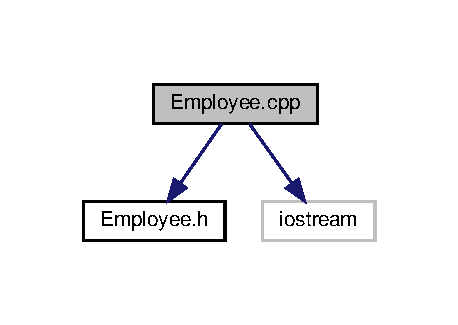
\includegraphics[width=220pt]{Employee_8cpp__incl}
\end{center}
\end{figure}


\subsection{Detailed Description}
Implementation of \hyperlink{classEmployee}{Employee}. 

\begin{DoxyAuthor}{Author}
Jackson Horton 
\end{DoxyAuthor}
\begin{DoxyDate}{Date}
2022-\/10-\/25 Implements all the functionality of the \hyperlink{classEmployee}{Employee} class. Some functionality is overriden by subclasses. 
\end{DoxyDate}

\hypertarget{Employee_8h}{}\section{Employee.\+h File Reference}
\label{Employee_8h}\index{Employee.\+h@{Employee.\+h}}


\hyperlink{classEmployee}{Employee} class; superclass to supervisor and officer.  


This graph shows which files directly or indirectly include this file\+:
\nopagebreak
\begin{figure}[H]
\begin{center}
\leavevmode
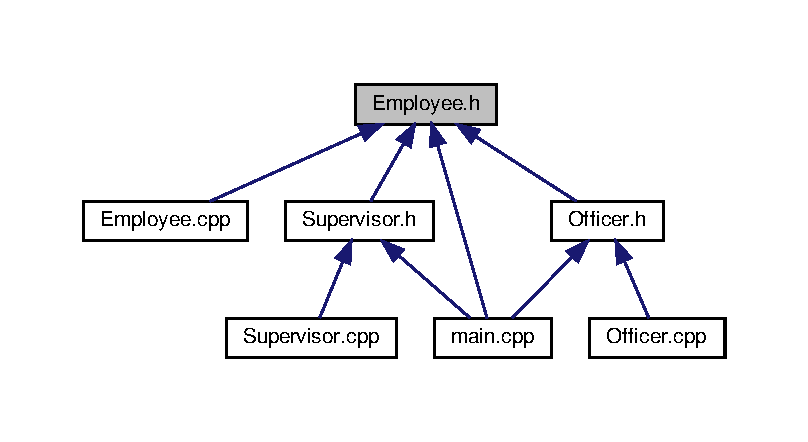
\includegraphics[width=350pt]{Employee_8h__dep__incl}
\end{center}
\end{figure}
\subsection*{Classes}
\begin{DoxyCompactItemize}
\item 
class \hyperlink{classEmployee}{Employee}
\begin{DoxyCompactList}\small\item\em \hyperlink{classEmployee}{Employee} class. \end{DoxyCompactList}\end{DoxyCompactItemize}


\subsection{Detailed Description}
\hyperlink{classEmployee}{Employee} class; superclass to supervisor and officer. 

\begin{DoxyAuthor}{Author}
Jackson Horton 
\end{DoxyAuthor}
\begin{DoxyDate}{Date}
2022-\/10-\/25 Contains all of the information pertaining to to a general employee. Subclasses contain specializations of this class. 
\end{DoxyDate}

\hypertarget{main_8cpp}{}\section{main.\+cpp File Reference}
\label{main_8cpp}\index{main.\+cpp@{main.\+cpp}}


Main function; facilitates class testing.  


{\ttfamily \#include $<$iostream$>$}\newline
{\ttfamily \#include \char`\"{}Employee.\+h\char`\"{}}\newline
{\ttfamily \#include \char`\"{}Supervisor.\+h\char`\"{}}\newline
{\ttfamily \#include \char`\"{}Officer.\+h\char`\"{}}\newline
Include dependency graph for main.\+cpp\+:
\nopagebreak
\begin{figure}[H]
\begin{center}
\leavevmode
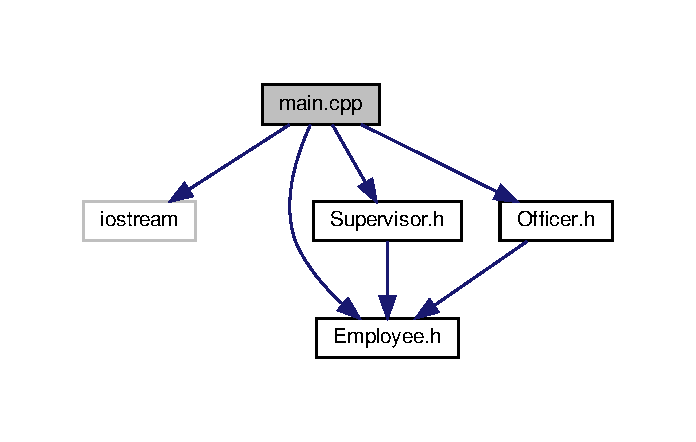
\includegraphics[width=334pt]{main_8cpp__incl}
\end{center}
\end{figure}
\subsection*{Functions}
\begin{DoxyCompactItemize}
\item 
\mbox{\Hypertarget{main_8cpp_a9ccea1912d6e2275d5612e294919d113}\label{main_8cpp_a9ccea1912d6e2275d5612e294919d113}} 
void {\bfseries run\+Employee\+Tests} (\hyperlink{classEmployee}{Employee} \&e)
\item 
\mbox{\Hypertarget{main_8cpp_ae66f6b31b5ad750f1fe042a706a4e3d4}\label{main_8cpp_ae66f6b31b5ad750f1fe042a706a4e3d4}} 
int {\bfseries main} ()
\end{DoxyCompactItemize}


\subsection{Detailed Description}
Main function; facilitates class testing. 

\begin{DoxyAuthor}{Author}
Jackson Horton 
\end{DoxyAuthor}
\begin{DoxyDate}{Date}
2022-\/10-\/25 In the main file, multiple \hyperlink{classEmployee}{Employee}, \hyperlink{classOfficer}{Officer}, and \hyperlink{classSupervisor}{Supervisor} objects are initialized. Then, their member funcitons are tested. 
\end{DoxyDate}

\hypertarget{Officer_8cpp}{}\section{Officer.\+cpp File Reference}
\label{Officer_8cpp}\index{Officer.\+cpp@{Officer.\+cpp}}


\hyperlink{classOfficer}{Officer} implementation.  


{\ttfamily \#include \char`\"{}Officer.\+h\char`\"{}}\newline
{\ttfamily \#include $<$iostream$>$}\newline
Include dependency graph for Officer.\+cpp\+:
\nopagebreak
\begin{figure}[H]
\begin{center}
\leavevmode
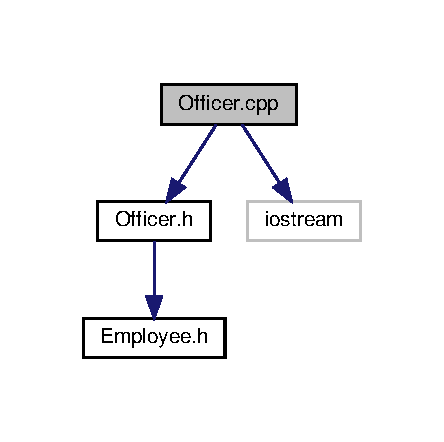
\includegraphics[width=213pt]{Officer_8cpp__incl}
\end{center}
\end{figure}


\subsection{Detailed Description}
\hyperlink{classOfficer}{Officer} implementation. 

\begin{DoxyAuthor}{Author}
Jackson Horton 
\end{DoxyAuthor}
\begin{DoxyDate}{Date}
2022-\/10-\/25 \hyperlink{classOfficer}{Officer} is a subclass of \hyperlink{classEmployee}{Employee}; alsoholds the officer\textquotesingle{}s evilness, which positively affects his pay. 
\end{DoxyDate}

\hypertarget{Officer_8h}{}\section{Officer.\+h File Reference}
\label{Officer_8h}\index{Officer.\+h@{Officer.\+h}}


\hyperlink{classOfficer}{Officer} class; represents an officer.  


{\ttfamily \#include \char`\"{}Employee.\+h\char`\"{}}\newline
Include dependency graph for Officer.\+h\+:
\nopagebreak
\begin{figure}[H]
\begin{center}
\leavevmode
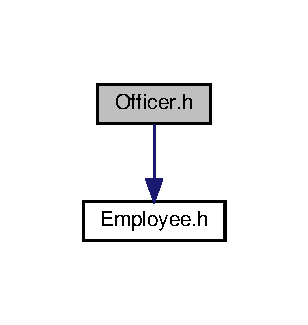
\includegraphics[width=148pt]{Officer_8h__incl}
\end{center}
\end{figure}
This graph shows which files directly or indirectly include this file\+:
\nopagebreak
\begin{figure}[H]
\begin{center}
\leavevmode
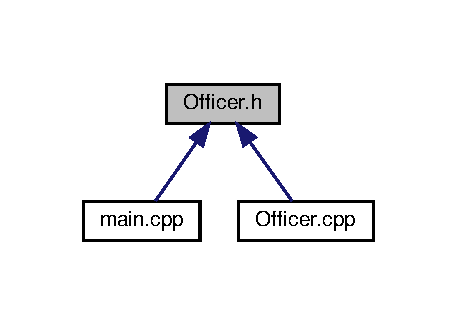
\includegraphics[width=220pt]{Officer_8h__dep__incl}
\end{center}
\end{figure}
\subsection*{Classes}
\begin{DoxyCompactItemize}
\item 
class \hyperlink{classOfficer}{Officer}
\end{DoxyCompactItemize}


\subsection{Detailed Description}
\hyperlink{classOfficer}{Officer} class; represents an officer. 

\begin{DoxyAuthor}{Author}
Jackson Horton 
\end{DoxyAuthor}
\begin{DoxyDate}{Date}
2022-\/10-\/25 Subclass of \hyperlink{classEmployee}{Employee}. Some member functions are overriden specifically to fit the officer class. 
\end{DoxyDate}

\hypertarget{Supervisor_8cpp}{}\section{Supervisor.\+cpp File Reference}
\label{Supervisor_8cpp}\index{Supervisor.\+cpp@{Supervisor.\+cpp}}


Implementation of \hyperlink{classSupervisor}{Supervisor} class.  


{\ttfamily \#include \char`\"{}Supervisor.\+h\char`\"{}}\newline
{\ttfamily \#include $<$iostream$>$}\newline
Include dependency graph for Supervisor.\+cpp\+:
\nopagebreak
\begin{figure}[H]
\begin{center}
\leavevmode
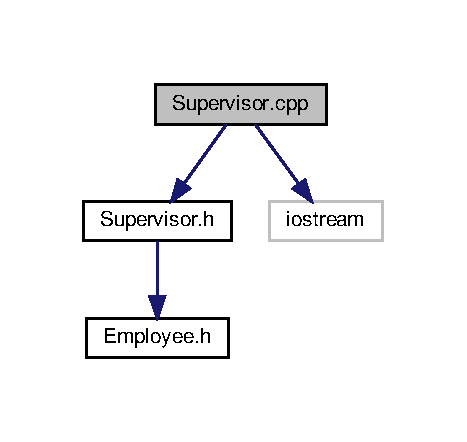
\includegraphics[width=224pt]{Supervisor_8cpp__incl}
\end{center}
\end{figure}


\subsection{Detailed Description}
Implementation of \hyperlink{classSupervisor}{Supervisor} class. 

\begin{DoxyAuthor}{Author}
Jackson Horton 
\end{DoxyAuthor}
\begin{DoxyDate}{Date}
2022-\/10-\/25 Subclass of employee. Implements/overrides some \hyperlink{classEmployee}{Employee} functions to be specific to the supervisor. 
\end{DoxyDate}

\hypertarget{Supervisor_8h}{}\section{Supervisor.\+h File Reference}
\label{Supervisor_8h}\index{Supervisor.\+h@{Supervisor.\+h}}


\hyperlink{classSupervisor}{Supervisor} class.  


{\ttfamily \#include \char`\"{}Employee.\+h\char`\"{}}\newline
Include dependency graph for Supervisor.\+h\+:
\nopagebreak
\begin{figure}[H]
\begin{center}
\leavevmode
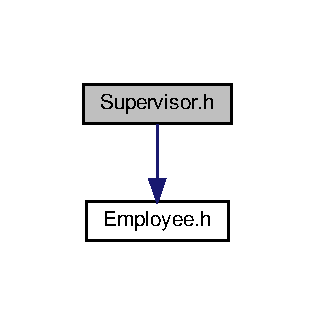
\includegraphics[width=151pt]{Supervisor_8h__incl}
\end{center}
\end{figure}
This graph shows which files directly or indirectly include this file\+:
\nopagebreak
\begin{figure}[H]
\begin{center}
\leavevmode
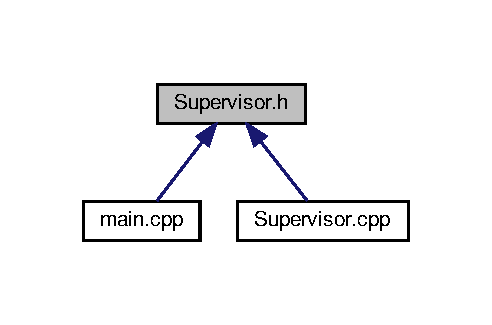
\includegraphics[width=236pt]{Supervisor_8h__dep__incl}
\end{center}
\end{figure}
\subsection*{Classes}
\begin{DoxyCompactItemize}
\item 
class \hyperlink{classSupervisor}{Supervisor}
\end{DoxyCompactItemize}


\subsection{Detailed Description}
\hyperlink{classSupervisor}{Supervisor} class. 

\begin{DoxyAuthor}{Author}
Jackson Horton 
\end{DoxyAuthor}
\begin{DoxyDate}{Date}
2022-\/10-\/25 \hyperlink{classSupervisor}{Supervisor} is a subclass of \hyperlink{classEmployee}{Employee} with some methods\textquotesingle{} implementation overriding \hyperlink{classEmployee}{Employee}\textquotesingle{}s to fit a supervisor. Also has more member variables, like number of people supervised.. 
\end{DoxyDate}

%--- End generated contents ---

% Index
\backmatter
\newpage
\phantomsection
\clearemptydoublepage
\addcontentsline{toc}{chapter}{Index}
\printindex

\end{document}
